\documentclass[]{article}
\usepackage{lmodern}
\usepackage{amssymb,amsmath}
\usepackage{ifxetex,ifluatex}
\usepackage{fixltx2e} % provides \textsubscript
\ifnum 0\ifxetex 1\fi\ifluatex 1\fi=0 % if pdftex
  \usepackage[T1]{fontenc}
  \usepackage[utf8]{inputenc}
\else % if luatex or xelatex
  \ifxetex
    \usepackage{mathspec}
  \else
    \usepackage{fontspec}
  \fi
  \defaultfontfeatures{Ligatures=TeX,Scale=MatchLowercase}
\fi
% use upquote if available, for straight quotes in verbatim environments
\IfFileExists{upquote.sty}{\usepackage{upquote}}{}
% use microtype if available
\IfFileExists{microtype.sty}{%
\usepackage{microtype}
\UseMicrotypeSet[protrusion]{basicmath} % disable protrusion for tt fonts
}{}
\usepackage[margin=1in]{geometry}
\usepackage{hyperref}
\hypersetup{unicode=true,
            pdftitle={PCBs sampling desgin summary},
            pdfauthor={Xuelong Wang},
            pdfborder={0 0 0},
            breaklinks=true}
\urlstyle{same}  % don't use monospace font for urls
\usepackage{graphicx,grffile}
\makeatletter
\def\maxwidth{\ifdim\Gin@nat@width>\linewidth\linewidth\else\Gin@nat@width\fi}
\def\maxheight{\ifdim\Gin@nat@height>\textheight\textheight\else\Gin@nat@height\fi}
\makeatother
% Scale images if necessary, so that they will not overflow the page
% margins by default, and it is still possible to overwrite the defaults
% using explicit options in \includegraphics[width, height, ...]{}
\setkeys{Gin}{width=\maxwidth,height=\maxheight,keepaspectratio}
\IfFileExists{parskip.sty}{%
\usepackage{parskip}
}{% else
\setlength{\parindent}{0pt}
\setlength{\parskip}{6pt plus 2pt minus 1pt}
}
\setlength{\emergencystretch}{3em}  % prevent overfull lines
\providecommand{\tightlist}{%
  \setlength{\itemsep}{0pt}\setlength{\parskip}{0pt}}
\setcounter{secnumdepth}{5}
% Redefines (sub)paragraphs to behave more like sections
\ifx\paragraph\undefined\else
\let\oldparagraph\paragraph
\renewcommand{\paragraph}[1]{\oldparagraph{#1}\mbox{}}
\fi
\ifx\subparagraph\undefined\else
\let\oldsubparagraph\subparagraph
\renewcommand{\subparagraph}[1]{\oldsubparagraph{#1}\mbox{}}
\fi

%%% Use protect on footnotes to avoid problems with footnotes in titles
\let\rmarkdownfootnote\footnote%
\def\footnote{\protect\rmarkdownfootnote}

%%% Change title format to be more compact
\usepackage{titling}

% Create subtitle command for use in maketitle
\providecommand{\subtitle}[1]{
  \posttitle{
    \begin{center}\large#1\end{center}
    }
}

\setlength{\droptitle}{-2em}

  \title{PCBs sampling desgin summary}
    \pretitle{\vspace{\droptitle}\centering\huge}
  \posttitle{\par}
    \author{Xuelong Wang}
    \preauthor{\centering\large\emph}
  \postauthor{\par}
      \predate{\centering\large\emph}
  \postdate{\par}
    \date{2020-01-13}

\usepackage{float,amsmath, bbm, siunitx, bm}
\usepackage{pdfpages}
\floatplacement{figure}{H}
\newcommand{\indep}{\rotatebox[origin=c]{90}{$\models$}}

\begin{document}
\maketitle

{
\setcounter{tocdepth}{2}
\tableofcontents
}
\section{PCBs data summary}\label{pcbs-data-summary}

There are 3 surveys were conducted during the 6 years from 1999-2014.
The number of PCBs which are measured are varied from each survey.
Besides, the measurement sensitivity were improved along the time. There
are some details of the PCBs measurements can be found in
\href{https://www.epa.gov/sites/production/files/2015-06/documents/ace3pcbreviewpackage3-02-11.pdf}{\textbf{\textbf{this
one}}} at page 3.

Another thing is the NHANES adopted a sub-sampling method after 2005 for
PCBs measurements. It seems that they collect all the blood samples from
all the subjects but they only chose a sub-sample of them to measure the
PCBs value. The details of the pool sampling method can be found in this
\href{https://wwwn.cdc.gov/Nchs/Nhanes/2005-2006/PCBPOL_D.htm}{\textbf{\textbf{this
one}}}. The basic idea is following:

\begin{enumerate}
\def\labelenumi{\arabic{enumi}.}
\tightlist
\item
  Divide the whole subjects into 32 demographic groups\\
\item
  For all the subjects in each demographic group, split them into pools
  with sample size around 8. Note that the number of pools are
  proportion to the total number of subjects in the demographic group.\\
\item
  Draw a random sample from each pools, so that those sub-samples keeps
  same pattern in term of demographic groups ratio.
\end{enumerate}

The following is a summary table of sub-samples of 2005-2006 subjects'
for getting PCBs measurements.
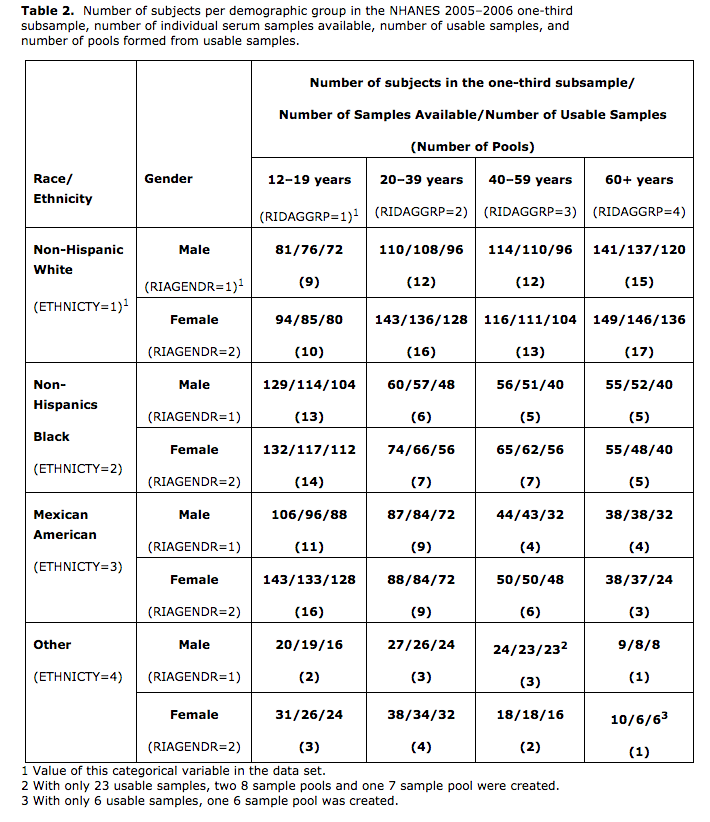
\includegraphics{./figs/subsampling_2005.png}

\newpage

Followings are some brief summary of the PCBs data.

\subsection{1999-2004}\label{section}

The types of PCBs measured for each survey is

\begin{verbatim}
$`1999`
 [1] "PCB028" "PCB052" "PCB066" "PCB074" "PCB099" "PCB101" "PCB105" "PCB118" "PCB128" "PCB138"
[11] "PCB146" "PCB153" "PCB156" "PCB157" "PCB167" "PCB170" "PCB172" "PCB177" "PCB178" "PCB180"
[21] "PCB183" "PCB187"

$`2001`
 [1] "PCB052" "PCB066" "PCB074" "PCB087" "PCB099" "PCB101" "PCB105" "PCB110" "PCB118" "PCB128"
[11] "PCB138" "PCB146" "PCB149" "PCB151" "PCB153" "PCB156" "PCB157" "PCB167" "PCB170" "PCB172"
[21] "PCB177" "PCB178" "PCB180" "PCB183" "PCB187" "PCB189" "PCB194" "PCB195" "PCB196" "PCB199"
[31] "PCB206"

$`2003`
 [1] "PCB028" "PCB066" "PCB074" "PCB105" "PCB118" "PCB156" "PCB157" "PCB167" "PCB189" "PCB044"
[11] "PCB049" "PCB052" "PCB087" "PCB099" "PCB101" "PCB110" "PCB128" "PCB138" "PCB146" "PCB149"
[21] "PCB151" "PCB153" "PCB170" "PCB172" "PCB177" "PCB178" "PCB180" "PCB183" "PCB187" "PCB194"
[31] "PCB195" "PCB196" "PCB199" "PCB206" "PCB209"
\end{verbatim}

The common PCBs that were measured by each survey is

\begin{verbatim}
 [1] "PCB052" "PCB066" "PCB074" "PCB099" "PCB101" "PCB105" "PCB118" "PCB128" "PCB138" "PCB146"
[11] "PCB153" "PCB156" "PCB157" "PCB167" "PCB170" "PCB172" "PCB177" "PCB178" "PCB180" "PCB183"
[21] "PCB187"
\end{verbatim}

I will use those 21 PCBs to calculate their covariance matrix.

The total number of PCBs data from 1999-2004 is 7106. After I remove all
the missing data, what I get is total 4873 observations.

\subsection{2005-2014}\label{section-1}

The types of PCBs measured for each survey is

\begin{verbatim}
$`2005`
 [1] "PCB028" "PCB044" "PCB049" "PCB052" "PCB066" "PCB074" "PCB087" "PCB099" "PCB101" "PCB105"
[11] "PCB110" "PCB114" "PCB118" "PCB123" "PCB128" "PCB138" "PCB146" "PCB149" "PCB151" "PCB153"
[21] "PCB156" "PCB157" "PCB167" "PCB170" "PCB172" "PCB177" "PCB178" "PCB180" "PCB183" "PCB187"
[31] "PCB189" "PCB194" "PCB195" "PCB196" "PCB199" "PCB206" "PCB209"

$`2007`
 [1] "PCB028" "PCB044" "PCB049" "PCB052" "PCB066" "PCB074" "PCB087" "PCB099" "PCB101" "PCB105"
[11] "PCB110" "PCB114" "PCB118" "PCB123" "PCB128" "PCB138" "PCB146" "PCB149" "PCB151" "PCB153"
[21] "PCB156" "PCB157" "PCB167" "PCB170" "PCB172" "PCB177" "PCB178" "PCB180" "PCB183" "PCB187"
[31] "PCB189" "PCB194" "PCB195" "PCB196" "PCB199" "PCB206" "PCB209"

$`2009`
 [1] "PCB028" "PCB066" "PCB074" "PCB099" "PCB105" "PCB114" "PCB118" "PCB138" "PCB146" "PCB153"
[11] "PCB156" "PCB157" "PCB167" "PCB170" "PCB178" "PCB180" "PCB183" "PCB187" "PCB189" "PCB194"
[21] "PCB196" "PCB199" "PCB206" "PCB209"

$`2011`
 [1] "PCB028" "PCB066" "PCB074" "PCB099" "PCB105" "PCB114" "PCB118" "PCB138" "PCB146" "PCB153"
[11] "PCB156" "PCB157" "PCB167" "PCB170" "PCB178" "PCB180" "PCB183" "PCB187" "PCB189" "PCB194"
[21] "PCB196" "PCB199" "PCB206" "PCB209"

$`2013`
 [1] "PCB028" "PCB066" "PCB074" "PCB099" "PCB105" "PCB114" "PCB118" "PCB138" "PCB146" "PCB153"
[11] "PCB156" "PCB157" "PCB167" "PCB170" "PCB178" "PCB180" "PCB183" "PCB187" "PCB189" "PCB194"
[21] "PCB196" "PCB199" "PCB206" "PCB209"
\end{verbatim}

The common PCBs that were measured by each survey is

\begin{verbatim}
 [1] "PCB028" "PCB066" "PCB074" "PCB099" "PCB105" "PCB114" "PCB118" "PCB138" "PCB146" "PCB153"
[11] "PCB156" "PCB157" "PCB167" "PCB170" "PCB178" "PCB180" "PCB183" "PCB187" "PCB189" "PCB194"
[21] "PCB196" "PCB199" "PCB206" "PCB209"
\end{verbatim}

I will use those 24 PCBs to calculate their covariance matrix.

The total number of PCBs data from 2005-2014 is 1347. After I remove all
the missing data, what I get is total 1228 observations.

Note that I only work on the PCBs measurement without adjustment, but I
used the under the limit adjustment.

\section{Some resource}\label{some-resource}

All the information of NHANES data could be found in their
\href{https://wwwn.cdc.gov/nchs/nhanes/}{\textbf{\textbf{webseit}}}, all
the information of PCBs are in the Laboratory data section, for example
\href{https://wwwn.cdc.gov/Nchs/Nhanes/2001-2002/L28POC_B.htm}{\textbf{\textbf{webseit}}}.


\end{document}
